\section{1174083 - Bakti Qilan Mufid}
Chapter-4 Klasifikasi Teks
\subsection{Teori}
\subsubsection{Jelaskan apa itu klasifikasi teks, sertakan gambar iustrasi buatan sendiri}
\hfill\\
Klasifikasi teks merupakan salah satu tugas terpenting dalam Pemrosesan Bahasa Alami (Natural Language Processing). Ini adalah proses mengklasifikasikan string teks atau dokumen ke dalam kategori yang berbeda, tergantung pada konten string. Klasifikasi teks memiliki berbagai aplikasi, seperti mendeteksi sentimen pengguna dari tweet, mengklasifikasikan email sebagai spam atau ham, mengklasifikasikan posting blog ke dalam kategori yang berbeda, penandaan otomatis permintaan pelanggan, dan sebagainya. BErikut adalah contoh dari Klasifikasi Teks. Contohnya, misal kita ingin mencari kata dog, is, table, on, the . kemudian jika kata yang dimaksud sesuai maka akan menampilkan bilangan biner 1 dan jika salah 0. Seperti dibawah ini :
\begin{figure}[H]
	\centering
	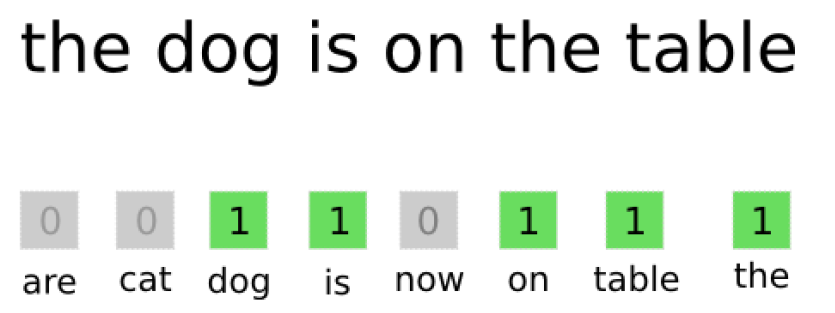
\includegraphics[width=8cm]{figures/1174083/figures4/1.png}
	\caption{Klasifikasi Teks}
\end{figure}

\subsubsection{Jelaskan mengapa klasifiasi bunga tidak bisa digunakan untuk machine learning, sertakan ilustrasi gambar sendiri}
\hfill\\
Dikarenakan tidak semua bunga memliki ciri - ciri yang sama. Atau dalam kata lain terdapat data noise dalam klasifikasi bunga sehingga tidak bisa menggunakan machine learning. Contohnya Anggrek memiliki warna ungu, dengan jumlah kelopak 5. Kemudian ada bunga warna ungu dengan jumlah kelopak yang sama namun ternyata bukan anggrek dan kategorinya banyak sekali. Bahkan ada bunga yang tidak jelas apakah warnanya sesuai atau tidak, sehingga bisa menyebabkan data noise.
\begin{figure}[H]
	\centering
	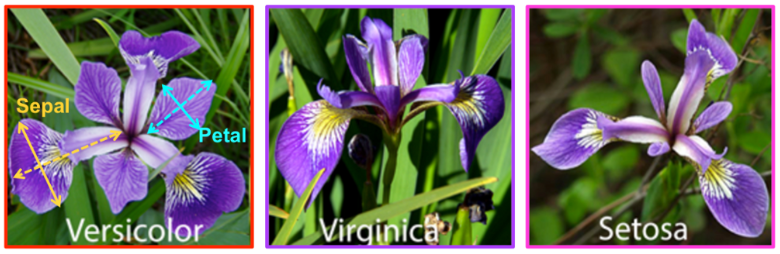
\includegraphics[width=8cm]{figures/1174083/figures4/2.png}
	\caption{Klasifikasi Bunga}
\end{figure}

\subsubsection{Jelaskan bagaimana teknik pembelajaran mesin pada teks pada kata-kata yang digunakan di youtube, jelaskan arti per atribut data csv dan sertakan ilustrasi buatan sendiri.}

\hfill\\
Menggunakan teknik bag-of-words pada klasifikasi berbasis text dan kata untuk mengklasifikasikan komentar yang ada di internet sebagai spam atau bukan. Misalkan pada kolom komentar dapat di cek seberapa sering suatu kata muncul dalam kalimat. Setiap kata dapat dijadikan baris dan kolomnya ini merupakan kategori kata terbut, apakah masuk kedalam spam atau tidak. dan contoh lainnya yaitu pada Caption. dimana akan muncul subtitle secara otomatis dari youtube menggunakan sensor suara yang disesuaikan dengan kata yang telah ditentukan. Contohnya seperti berikut :
\begin{figure}[H]
	\centering
	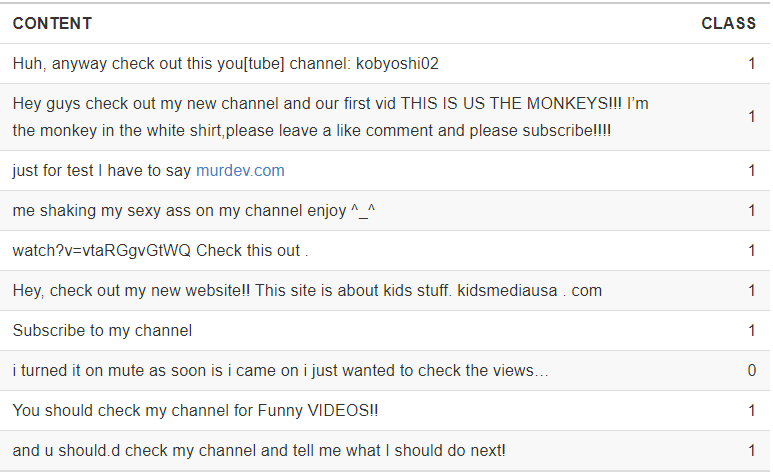
\includegraphics[width=8cm]{figures/1174083/figures4/3.png}
	\caption{Klasifikasi Spam Comment di Youtube}
\end{figure}

\subsubsection{Jelaskan apa yang dimaksud vektorisasi data.}
\hfill\\

Vektorisasi adalah proses konversi data raster(gambar, pindaian)  menjadi data vektor yang lebih umum disebut dengan istilah  digitalisasi adapun aktifitasnya disebut digitasi. Wujud digitalisasi ini diklasifikasikan secara spesifik dalam tema-tema tertentu yang direpresentasikan oleh bentuk garis, poligon dan titik. Pada akhirnya proses vektorisasi ini menghasilkan suatu wujud peta topografi yang menggambarkan keadaan permukaan bumi atau bentang alam. Sifat data yang geometris menunjukkan ukuran dimensi yang sesungguhnya.
\begin{figure}[H]
	\centering
	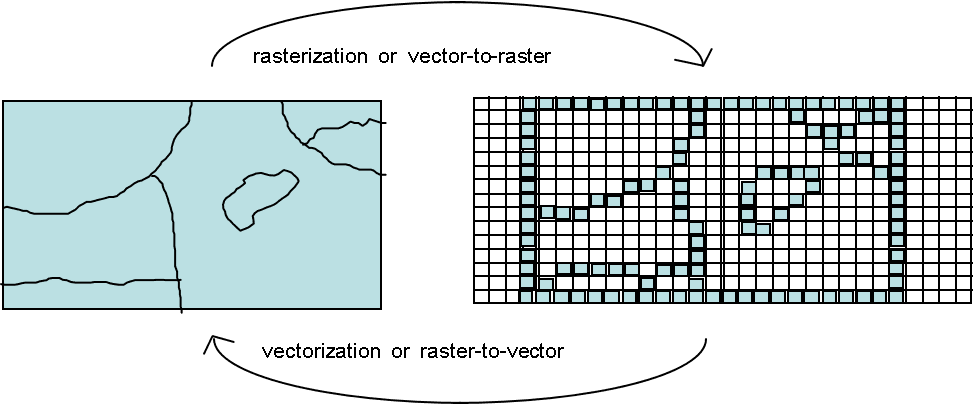
\includegraphics[width=8cm]{figures/1174083/figures4/5.png}
	\caption{Vektorisasi dan Rasterisasi}
\end{figure}

\subsubsection{Jelaskan apa itu bag of words dengan kata-kata yang sederhana dan ilustrasi sendiri.}
\hfill\\

bag-of-words merupakan representasi teks yang menggambarkan kemunculan kata-kata dalam dokumen. Pengelompokan kata kata kedalam perhitungan, berapakali sebuah kata muncul dalam satu kalimat. Disebut ”bag” katakata, karena informasi tentang susunan atau struktur kata dalam dokumen dibuang. Model ini hanya berkaitan dengan apakah kata-kata yang diketahui muncul dalam dokumen, bukan di mana dalam dokumen.
Contohnya disini akan melihat kemunculan kata dari kalimat :
\begin{enumerate}
\item I Love Dogs
\item I hate dogs and knitting
\item Knitting is my hobby and passion.
\end{enumerate}
\begin{figure}[H]
	\centering
	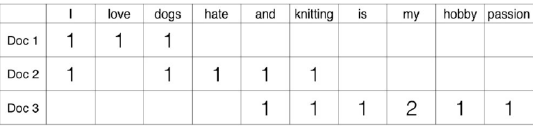
\includegraphics[width=8cm]{figures/1174083/figures4/4.png}
	\caption{Bag-Of-Words}
\end{figure}

\subsubsection{Jelaskan apa itu TF-IDF, ilustrasikan dengan gambar sendiri.}
\hfill\\

TF-IDF memberi kita frekuensi kata dalam setiap dokumen dalam korpus atau mengganti data jadi number. Ini adalah rasio berapa kali kata itu muncul dalam dokumen dibandingkan dengan jumlah total kata dalam dokumen itu. Itu meningkat seiring jumlah kemunculan kata itu di dalam dokumen meningkat. Setiap dokumen memiliki tf sendiri. Dalam ilustrasi disini saya akan mengganti contoh Bag of Words menjadi bentuk TF-IDF.

\begin{figure}[H]
	\centering
	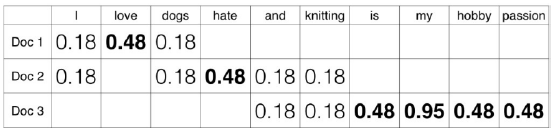
\includegraphics[width=8cm]{figures/1174083/figures4/6.png}
	\caption{Contoh TF-IDF}
\end{figure}

\subsection{Praktek}
\subsubsection{buat aplikasi klasifikasi sederhana menggunakan pandas, buat data dummy format csv sebanyak 500 baris dan melakukan load ke dataframe panda.jelaskan arti setiap baris kode yang dibuat(harus beda dengan teman sekelas)}
\hfill\\
\lstinputlisting[firstline=8, lastline=9, caption={kodingan praktek no. 1},captionpos=b]{src/1174083/src4/1174083.py}
	\begin{figure}[H]
	\centering
		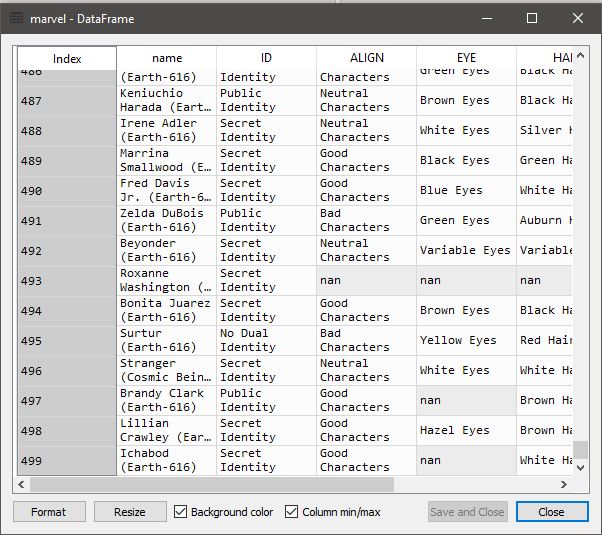
\includegraphics[width=8 cm]{figures/1174083/figures4/7.png}
	\caption{hasil praktek soal no. 1}
	\end{figure}


\subsubsection{dari dataframe tersebut dipecah menjadi dua dataframe yaitu 450 row pertama dan 50 row sisanya(harus beda dengan teman sekelas)}
\hfill\\
\lstinputlisting[firstline=11, lastline=11, caption={kodingan praktek no. 2},captionpos=b]{src/1174083/src4/1174083.py}
	\begin{figure}[H]
	\centering
		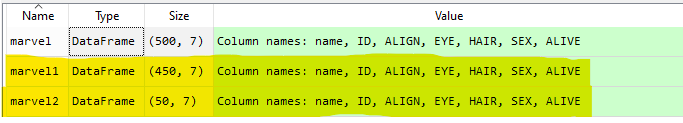
\includegraphics[width=8 cm]{figures/1174083/figures4/8.png}
	\caption{hasil praktek soal no. 2}
	\end{figure}

\subsubsection{praktekkan vektorisasi dan klasifikasi dari data(NPM mod 4, jika 0 maka ketty perry, 1 LMFAO, 2 Eminem, 3 Shakira) dengan Decission Tree. Tunjukkan keluaranya dari komputer sendiri dan artikan maksud luaran yang di dapatkan}
\hfill\\
\lstinputlisting[firstline=9, lastline=9, caption={1174083 mod 4},captionpos=b]{src/1174083/src4/1174083-2.py}

\lstinputlisting[firstline=12, lastline=36, caption={kodingan praktek no. 3},captionpos=b]{src/1174083/src4/1174083-2.py}
	\begin{figure}[H]
	\centering
		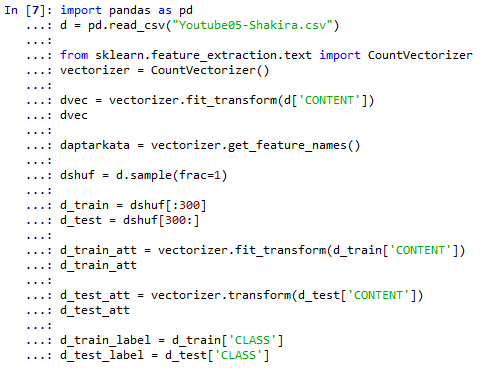
\includegraphics[width=8 cm]{figures/1174083/figures4/9.png}
	\caption{hasil praktek soal no. 3(1)}
	\end{figure}
	Vektorisasi data content dari file Youtube04\_Shakira.CSV
	\begin{figure}[H]
	\centering
		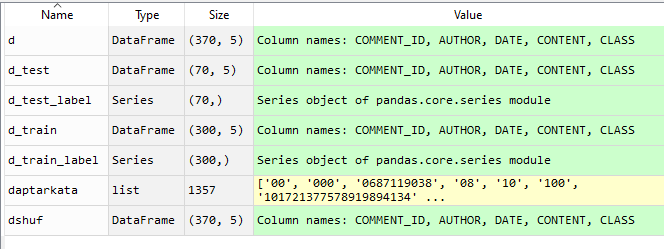
\includegraphics[width=8 cm]{figures/1174083/figures4/10.png}
	\caption{hasil praktek soal no. 3(2)}
	\end{figure}
	
\subsubsection{Cobalah klarifikasikan dari data vektorisasi yang di tentukan di nomor sebelumnya dengan klasifikasi SVM. Tunjukkan keluaranya dari komputer sendiri dan artikan maksud setiap luaran yang didapatkan}
\hfill\\
\lstinputlisting[firstline=47, lastline=50, caption={kodingan praktek no. 4},captionpos=b]{src/1174083/src4/1174083-2.py}
	\begin{figure}[H]
	\centering
		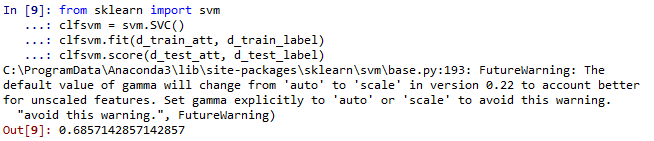
\includegraphics[width=8 cm]{figures/1174083/figures4/11.png}
	\caption{hasil praktek soal no. 4}
	\end{figure}

\subsubsection{Cobalah klasifikasikan dari data vektorisasi yang ditentukan dari nomor sebelumnya dengan klasifikasi Decision Tree. Tunjukan keluaranya dari komputer sendiri dan artikan maksud setiap luaran yang didapatkan}
\hfill\\
\lstinputlisting[firstline=40, lastline=43, caption={kodingan praktek no. 5},captionpos=b]{src/1174083/src4/1174083-2.py}
	\begin{figure}[H]
	\centering
		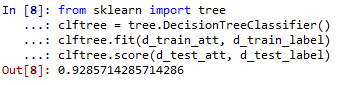
\includegraphics[width=8 cm]{figures/1174083/figures4/12.png}
	\caption{hasil praktek soal no. 5}
	\end{figure}

\subsubsection{Plotlah confusion matrix dari praktek modul ini menggunakan matplotlib.Tunjukkan keluarannya dari komputer sendiri dan artikan maksud setiap luaran yang didapatkan.}
\hfill\\
\lstinputlisting[firstline=61, lastline=106, caption={kodingan praktek no. 6(1)},captionpos=b]{src/1174083/src4/1174083-2.py}
	\begin{figure}[H]
	\centering
		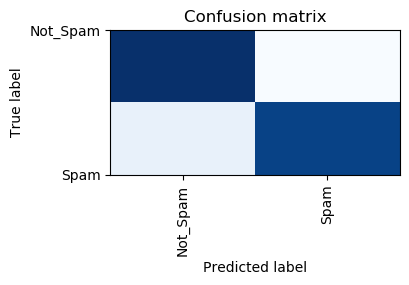
\includegraphics[width=8 cm]{figures/1174083/figures4/13.png}
	\caption{hasil praktek soal no. 6(1)}
	\end{figure}
	Plot confusion matrix dari klasifikasi Decission Tree.
\lstinputlisting[firstline=110, lastline=159, caption={kodingan praktek no. 6(2)},captionpos=b]{src/1174083/src4/1174083-2.py}
	\begin{figure}[H]
	\centering
		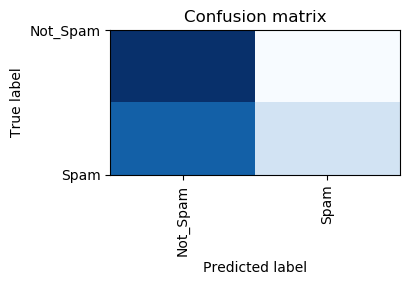
\includegraphics[width=8 cm]{figures/1174083/figures4/14.png}
	\caption{hasil praktek soal no. 6(2)}
	\end{figure}
	Plot confusion matrix dari klasifikasi SVM.
\lstinputlisting[firstline=163, lastline=211, caption={kodingan praktek no. 6(3)},captionpos=b]{src/1174083/src4/1174083-2.py}
	\begin{figure}[H]
	\centering
		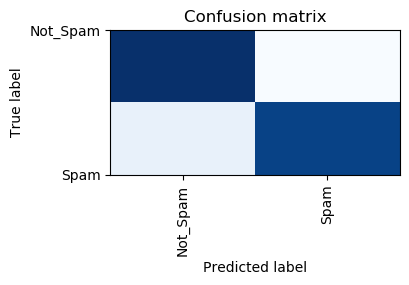
\includegraphics[width=8 cm]{figures/1174083/figures4/15.png}
	\caption{hasil praktek soal no. 6(3)}
	\end{figure}
	Plot confusion matrix dari klasifikasi Random Forest.
	
\subsubsection{jalankan program cross validaiton pada bagian teori bab ini. Tunjukkan keluarannya dari komputer sendiri dan artikan maksud setiap luaran yang didapatkan.}
\hfill\\
\lstinputlisting[firstline=215, lastline=224, caption={kodingan praktek no. 7},captionpos=b]{src/1174083/src4/1174083-2.py}
	\begin{figure}[H]
	\centering
		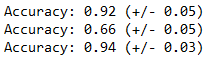
\includegraphics[width=5 cm]{figures/1174083/figures4/16.png}
	\caption{hasil praktek soal no. 7}
	\end{figure}

\subsubsection{Buatlah program pengamatan komponen informasi pada bagian teori bab ini. Tunjukkan keluarannya dari komputer sendiri dan artikan maksud setiap luaran yang didapatkan.}
\hfill\\
\lstinputlisting[firstline=228, lastline=241, caption={kodingan praktek no. 8},captionpos=b]{src/1174083/src4/1174083-2.py}
	\begin{figure}[H]
	\centering
		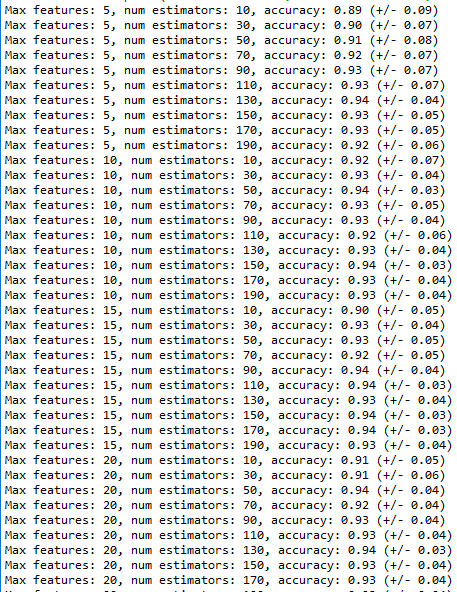
\includegraphics[width=8 cm]{figures/1174083/figures4/17.png}
	\caption{hasil praktek soal no. 8(1)}
	\end{figure}
	\hfill\\
	\begin{figure}[H]
	\centering
		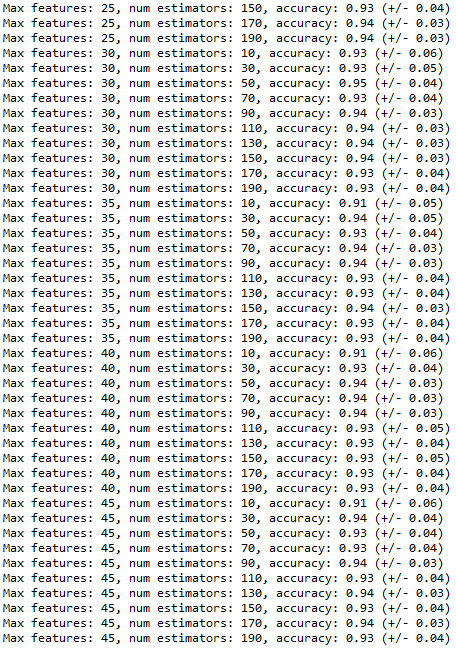
\includegraphics[width=8 cm]{figures/1174083/figures4/18.png}
	\caption{hasil praktek soal no. 8(2)}
	\end{figure}
	
\subsection{Penanganan Error}
pada chapter 4 ini saya tidak menemukan error.

\subsection{Bukti Tidak Plagiat}
\begin{figure}[H]
	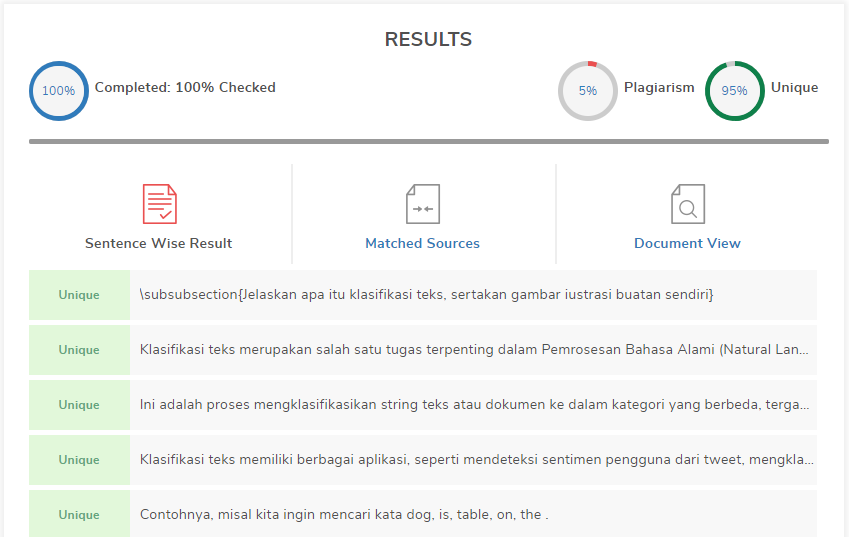
\includegraphics[width=10cm]{figures/1174083/figures4/20.png}
	\centering
	\caption{Bukti tidak plagiat}
\end{figure}

\subsection{Link Youtube}
https://youtu.be/la8Jptbm3Mo